\newpage
\section{Introduction}
\todo[inline]{/{This section shall introduce the reader to the subject addressed by the report. It should include i) a brief explanation of how a brake-by-wire system works and its main advantages and drawbacks compared to existing brake systems, and ii) a description of the purpose of the report, i.e., a formulation of the problem to which the report provides an answer. The last paragraph should consist of a “roadmap” of the report.}/}

%The aim of this laboratory class is to show how dependability modelling can be used to compare different design solutions for a fault-to lerant system. We will compare two candidate architectures for a brake-by-wire system. 

%Brake-by-wire systems are expected to repl ace hydraulic brake systems in future road vehicles. In a brake-by-wire system, the drive r’s brake intention is transmitted electronically from the brake pedal to electro-hydraulic or electro-mechanical brake actuators positioned at each wheel. Potential advantages of brake-by-wire systems compared to traditional hydraulic systems include lower cost, lower weight and simpler integration with stability control and active safety systems. 

%Figure 1 shows an overview of the brake-by-wire system. The brake pedal is connected to a central unit (CU). When the driver presses th e brake pedal, the central unit sends messages containing brake commands to each of the four wh eel units (WU). To ensure the safety of the system, the central unit and the wheel units must be fault-tolerant. Both the central unit and the wheel units are therefore implemented us ing redundant computer modules (see Figure 3 and 4). Two serial busses (SB1 and SB2) are pr ovided to ensure fault-tolerance for the data communication. 

%To optimize brake performance, the system executes a closed loop anti-lock braking control algorithm for each wheel. The inputs to the anti-lo ck control program consist of the current wheel speed and brake force commands genera ted by a stability control program, which is executed in the central unit. The wheel speed is measured by a wheel speed sensor included in each wheel unit. The input to the stability control program consists of data from several sensors. These sensors measures the position of th e brake-pedal (the driver’s brake intention), the angle of the steering wheel (the driver’s inte nded direction), the yaw rate (the rotation rate of the vehicle around its y-axis), the roll rate , and the vehicle’s lateral and longitudinal acceleration. In this laboratory class, we will fo cus our attention on where to execute the anti- lock-braking algorithms. We will not consider the reliability of the sensors used by stability control program.  



\begin{figure}[h!]
  \centering
  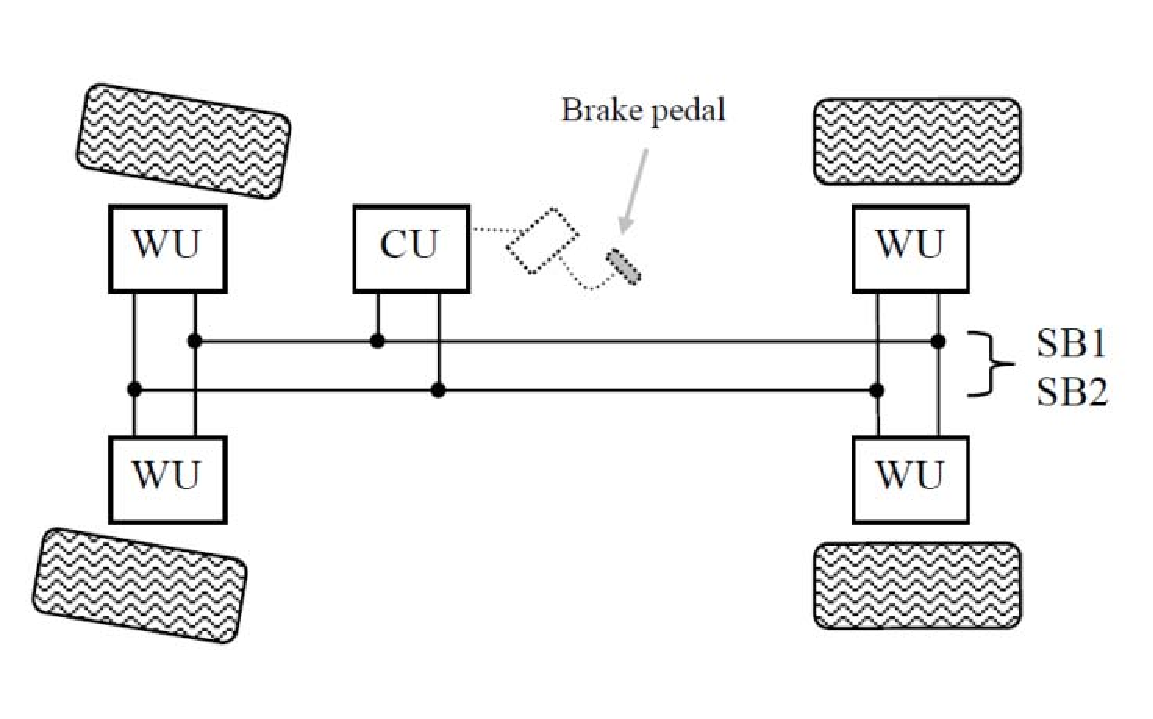
\includegraphics[scale=.5]{Fig1.pdf}
  \caption{Brake-by-wire system}
  \label{fig1}
\end{figure}